\chapter{EG-X Model}\label{ch:eg-x-model}

\section{Lattice Structure of Graphene}\label{sec:lattice-structure-of-graphene}

Following~\cite{Yang_Li_Lee_Ng_2018}.

Monolayer graphene forms a hexagonal lattice.
This is formed by two triangular sub lattices.
So in the unit cell of the hexagonal actually has two atoms.

Primitive lattice vectors of the hexagonal lattice:
\begin{align}
    \vb{a}_1 &= \frac{a}{2} \begin{pmatrix} 1 \\ \sqrt{3} \end{pmatrix} \\
    \vb{a}_2 &= \frac{a}{2} \begin{pmatrix} 1 \\ -\sqrt{3} \end{pmatrix}
\end{align}
with lattice constant \(a \approx \SI{2.46}{\angstrom}\) (distance between unit cells).
Have
\begin{equation}
    a = \sqrt{3} a_0
\end{equation}
with the nearest-neighbour distance \(a_0\).

\begin{figure}[htb]
    \centering
    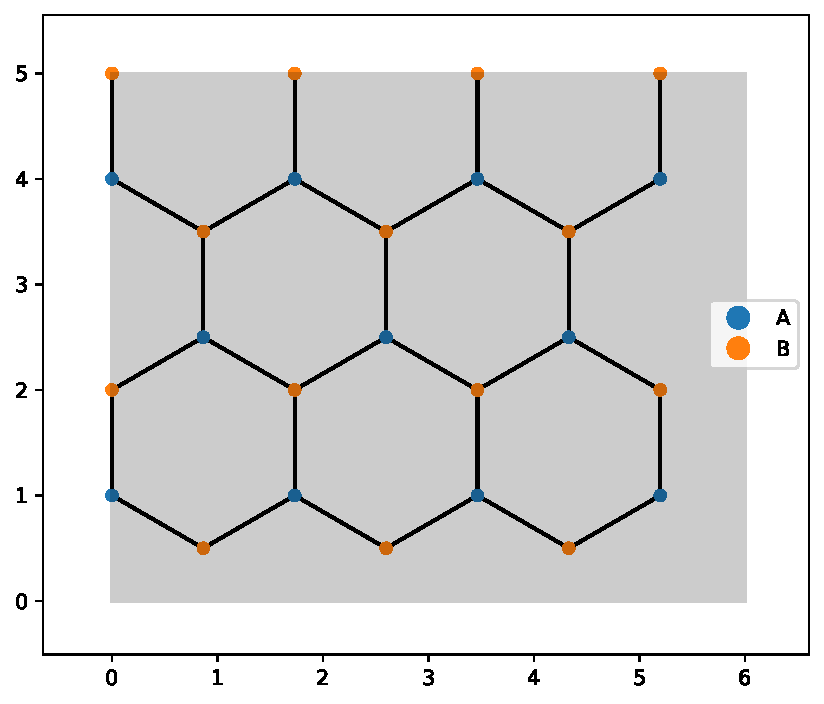
\includegraphics[width=0.7\textwidth]{images/graphene lattice}
    \caption{Graphene lattice structure}
    \label{fig:graphene lattice structure}
\end{figure}

Vectors to the nearest-neighbor \(B_i\) (\(i = 1, 2, 3,\)) atoms from atom \(A\):
\begin{align}
    \vb{\delta}_{AB, 1} = \begin{pmatrix} 0 \\ \frac{a}{\sqrt{3}} \end{pmatrix}, \vb{\delta}_{AB, 2} = \begin{pmatrix} \frac{a}{2} \\ -\frac{a}{2\sqrt{3}} \end{pmatrix}, \vb{\delta}_{AB, 3} = \begin{pmatrix} -\frac{a}{2} \\ -\frac{a}{2\sqrt{3}} \end{pmatrix}
\end{align}

Vectors to the nearest-neighbor \(A_i\) (\(i = 1, 2, 3,\)) atoms from atom \(B\):
\begin{align}
    \vb{\delta}_{BA, 1} = \begin{pmatrix} 0 \\ -\frac{a}{\sqrt{3}} \end{pmatrix}, \vb{\delta}_{BA, 2} = \begin{pmatrix} \frac{a}{2} \\ \frac{a}{2\sqrt{3}} \end{pmatrix}, \vb{\delta}_{BA, 3} = \begin{pmatrix} -\frac{a}{2} \\ \frac{a}{2\sqrt{3}} \end{pmatrix}
\end{align}

The vectors between the Graphene \(\mathrm{A}\) atom and the six neighbours on the same sub lattice can be found by rotating \(\vb{a}_1\) six times by \(\nicefrac{1}{6} * 2\pi = \nicefrac{\pi}{3}\):
\begin{align}
    \vb{\delta}_{AA, 1} &= \vb{a}_1 = \frac{a}{2} \begin{pmatrix} 1 \\ \sqrt{3} \end{pmatrix} = a \begin{pmatrix} \frac{1}{2} \\ \frac{\sqrt{3}}{2} \end{pmatrix} = a \begin{pmatrix} \sin{(\frac{\pi}{6})} \\ \cos{(\frac{\pi}{6})} \end{pmatrix} \\
    \vb{\delta}_{AA, 2} &= a \begin{pmatrix} \sin{(\frac{3\pi}{6})} \\ \cos{(\frac{3\pi}{6})} \end{pmatrix} = a \begin{pmatrix} 1 \\ 0 \end{pmatrix} \\
    \vb{\delta}_{AA, 3} &= a \begin{pmatrix} \sin{(\frac{5\pi}{6})} \\ \cos{(\frac{5\pi}{6})} \end{pmatrix} = a \begin{pmatrix} \frac{1}{2} \\ -\frac{\sqrt{3}}{2} \end{pmatrix} \\
    \vb{\delta}_{AA, 4} &= a \begin{pmatrix} \sin{(\frac{7\pi}{6})} \\ \cos{(\frac{7\pi}{6})} \end{pmatrix} = a \begin{pmatrix} -\frac{1}{2} \\ -\frac{\sqrt{3}}{2} \end{pmatrix} \\
    \vb{\delta}_{AA, 5} &= a \begin{pmatrix} \sin{(\frac{9\pi}{6})} \\ \cos{(\frac{9\pi}{6})} \end{pmatrix} = a \begin{pmatrix} -1 \\ 0 \end{pmatrix} \\
    \vb{\delta}_{AA, 6} &= a \begin{pmatrix} \sin{(\frac{11\pi}{6})} \\ \cos{(\frac{11\pi}{6})} \end{pmatrix} = a \begin{pmatrix} -\frac{1}{2} \\ \frac{\sqrt{3}}{2} \end{pmatrix}
\end{align}

\begin{figure}[htb]
    \centering
    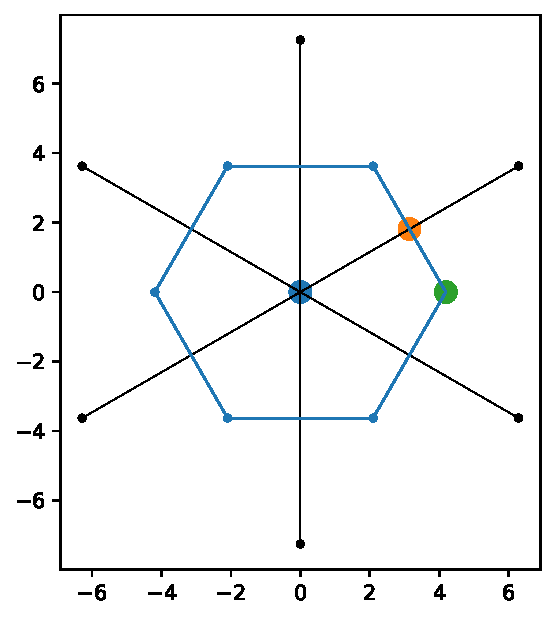
\includegraphics[width=0.5\textwidth]{images/graphene brillouin_zone}
    \caption{Graphene Brillouin Zone}
    \label{fig:graphene Brillouin zone}
\end{figure}

The primitive reciprocal lattice vectors \(\vb{b}_1\), \(\vb{b}_2\) fulfill
\begin{align}
    \vb{a}_1 \cdot \vb{b}_1 &= \vb{a}_2 \cdot \vb{b}_2 = 2\pi \\
    \vb{a}_1 \cdot \vb{b}_2 &= \vb{a}_2 \cdot \vb{b}_1 = 0
    \;,
\end{align}
so we have:
\begin{align}
    \vb{b}_1 &= \frac{2\pi}{a} \begin{pmatrix} 1 \\ \frac{1}{\sqrt{3}} \end{pmatrix} \\
    \vb{b}_2 &= \frac{2\pi}{a} \begin{pmatrix} 1 \\ - \frac{1}{\sqrt{3}} \end{pmatrix}
\end{align}
Points of high symmetry in the Brillouin zone are:
\begin{align}
    \Gamma &= \begin{pmatrix} 0 \\ 0 \end{pmatrix} \\
    \mathrm{M} &= \frac{\pi}{a} \begin{pmatrix} 1 \\ \frac{1}{\sqrt{3}} \end{pmatrix} \\
    \mathrm{K} &= \frac{4\pi}{3 a} \begin{pmatrix} 1 \\ 0 \end{pmatrix}
\end{align}


\section{EG-X Model}\label{sec:eg-x-model}

Graphene lattice and a site X\@.
\begin{figure}[htb]
    \centering
    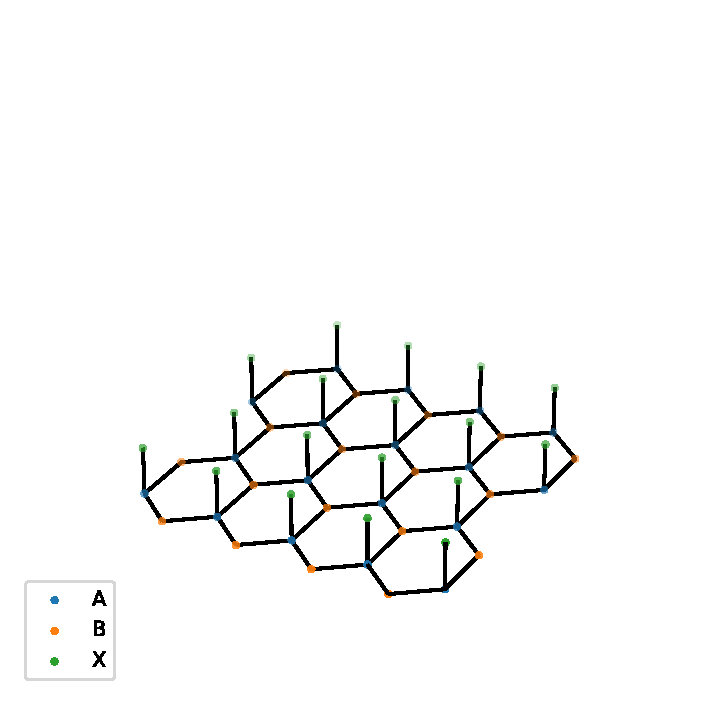
\includegraphics[width=0.5\textwidth]{images/eg-x lattice}
    \caption{EG-X model}
    \label{fig:eg-x model}
\end{figure}
Real-life motivation: layer of graphene on top of a substrate of another material (which provides the additional X atoms).
There is no spin-orbit coupling considered in the model (according to Niklas) when mapping to substrates Sn or Pb, it could be necessary (but does not the qualitative result?).

Without interaction \todo{Spin-orbit coupling, drop second spin index?}:
\begin{equation}
    H_0 = -t_{\mathrm{X}} \sum_{\langle ij \rangle, \sigma \sigma^{\prime}} d_{i, \sigma}^{\dagger} d_{j, \sigma^{\prime}}
    -t_{\mathrm{Gr}} \sum_{\langle ij \rangle, \sigma \sigma^{\prime}} \left(
    c_{i, \sigma}^{(A), \dagger} c_{j, \sigma^{\prime}}^{(B)} +
    c_{j, \sigma^{\prime}}^{(B), \dagger} c_{i, \sigma}^{(A)}
    \right)
    + V \sum_{i, \sigma \sigma^{\prime}} \left(
    d_{i, \sigma}^{\dagger} c_{i, \sigma^{\prime}}^{(A)} +
    c_{i, \sigma}^{(A), \dagger} d_{i, \sigma^{\prime}}
    \right)
    \label{eq:EG-X model Hamiltonian non-interacting}
\end{equation}
with:
\begin{itemize}
    \item \(d\) operators on the X atom
    \item \(c^{(\epsilon)}\) operators on the graphene site (\(\epsilon = A, B\))
    \item \(t_X\) NN hopping for X
    \item \(t_{Gr}\) NN hopping of Gr
    \item \(V\) hybridization between \(\mathrm{X}\) and Graphene \(\mathrm{B}\) sites
\end{itemize}
We can also introduce an onsite Hubbard interaction:
\begin{equation}
    H_{\mathrm{int}} = U_{\mathrm{X}} \sum_{i} d_{i, \uparrow}^{\dagger} d_{i, \downarrow}^{\dagger} d_{i, \downarrow} d_{i, \uparrow}
    + U_{\mathrm{Gr}} \sum_{i, \epsilon=A, B} c_{i, \uparrow}^{(\epsilon) \dagger} c_{i, \downarrow}^{(\epsilon) \dagger} c_{i, \downarrow}^{\epsilon} c_{i, \uparrow}^{\epsilon}
\end{equation}

\subsection{Band structure of the non-interacting EG-X model}\label{subsec:band-structure-of-the-non-interacting-eg-x-model}

To treat eq.~\ref{eq:EG-X model Hamiltonian non-interacting}, we first write out the sums over nearest neighbours \(\langle i, j \rangle\) explicitly, writing \(\vb{\delta}_{\mathrm{X}}, \vb{\delta}_{\epsilon}\) (\(\epsilon = A, B\)) for the connections to the nearest neighbours of the \(\mathrm{X}\) atoms and Graphene \(A, B\) sites.
Doing the calculation for the example of the \(\mathrm{X}\) atoms:
\begin{align}
    -t_{\mathrm{X}} \sum_{\langle ij \rangle, \sigma \sigma^{\prime}} d_{i, \sigma}^{\dagger} d_{j, \sigma^{\prime}}
    &= -\frac{t_X}{2} \sum_{i,\sigma, \sigma^{\prime}} \sum_{\delta_{\mathrm{X}}} d_{i, \sigma}^{\dagger} d_{i + \delta_{\mathrm{X}}, \sigma^{\prime}} \label{eq:EG-X model X atoms nearest neighbours written out} \\
\end{align}
(The factor \(\nicefrac{1}{2}\) is to account for double counting when going to the sum over all lattice sites \(i\))

Now we can input the discrete Fourier transform (for both graphene and X operators) into eq.~\ref{eq:EG-X model X atoms nearest neighbours written out}
\begin{align}
    c_{i} &= \frac{1}{\sqrt{N}} \sum_{\vb{k}} e^{\iu \vb{k} \vb{r}_{i}} c_{\vb{k}} \\
    c_{i}^{\dagger} &= \frac{1}{\sqrt{N}} \sum_{\vb{k}} e^{-\iu \vb{k} \vb{r}_{i}} c_{\vb{k}}^{\dagger}
\end{align}
with the completeness relation:
\begin{equation}
    \sum_{i} e^{\iu \vb{k} \vb{r}_{i}} e^{-\iu \vb{k}^{\prime} \vb{r}_{i}} = N \delta_{\vb{k}, \vb{k}^{\prime}}
    \;.
\end{equation}
We get:
\begin{align}
    -\frac{t_X}{2} \frac{1}{N} \sum_{i,\sigma, \sigma^{\prime}} \sum_{\vb{\delta}_{\mathrm{X}}} d_{i, \sigma}^{\dagger} d_{i + \vb{\delta}_{\mathrm{X}}, \sigma^{\prime}}
    &= -\frac{t_X}{2} \frac{1}{N} \sum_{i,\sigma, \sigma^{\prime}} \sum_{\vb{\delta}_{\mathrm{X}}} \sum_{\vb{k}, \vb{k}^{\prime}} e^{-\iu \vb{k} \vb{r}_i} d_{\vb{k}, \sigma}^{\dagger} e^{\iu \vb{k}^{\prime} \vb{r}_i} e^{\iu \vb{k}^{\prime} \vb{\delta}_{\mathrm{X}}} d_{\vb{k}^{\prime}, \sigma^{\prime}} \\
    &= -\frac{t_X}{2} \frac{1}{N} \sum_{\vb{k}, \vb{k^{\prime}}, \sigma, \sigma^{\prime}} \sum_{\vb{\delta}_{\mathrm{X}}} d_{\vb{k}, \sigma}^{\dagger}  e^{\iu \vb{k}^{\prime} \vb{\delta}_{\mathrm{X}}} d_{\vb{k}^{\prime}, \sigma^{\prime}} \sum_{i} e^{-\iu \vb{k} \vb{r}_i} e^{\iu \vb{k}^{\prime} \vb{r}_i} \\
    &= -\frac{t_X}{2} \frac{1}{N} \sum_{\vb{k}, \vb{k^{\prime}}, \sigma, \sigma^{\prime}} \sum_{\vb{\delta}_{\mathrm{X}}} d_{\vb{k}, \sigma}^{\dagger}  e^{\iu \vb{k}^{\prime} \vb{\delta}_{\mathrm{X}}} d_{\vb{k}^{\prime}, \sigma^{\prime}} N \delta_{\vb{k}, \vb{k}^{\prime}} \\
    &= -\frac{t_X}{2} \sum_{\vb{k}, \sigma, \sigma^{\prime}}  d_{\vb{k}, \sigma}^{\dagger}d_{\vb{k}, \sigma^{\prime}} \sum_{\vb{\delta}_{\mathrm{X}}} e^{\iu \vb{k} \vb{\delta}_{\mathrm{X}}}
\end{align}
The nearest neighbours for \(\mathrm{X}\) atoms are the vectors \(\vb{\delta}_{AA, i}\) from section~\ref{sec:lattice-structure-of-graphene}.
With that, we can calculate:
\begin{align}
    f_{\mathrm{X}} (\vb{k}) &= -\frac{t_X}{2} \sum_{\vb{\delta}_{\mathrm{X}}} e^{\iu \vb{k} \vb{\delta}_{\mathrm{X}}} \\
    &= -\frac{t_X}{2} \left( e^{\iu a (\frac{k_x}{2} + \frac{\sqrt{3} k_y}{2})}
    + e^{\iu a k_x}
    + e^{\iu a (\frac{k_x}{2} - \frac{\sqrt{3} k_y}{2})}
    \right. \\
    &+ \left. e^{\iu a (-\frac{k_x}{2} - \frac{\sqrt{3} k_y}{2})}
    + e^{-\iu a k_x}
    + e^{\iu a (-\frac{k_x}{2} + \frac{\sqrt{3} k_y}{2})} \right) \\
    &= -\frac{t_X}{2} \left( 2 \cos{(a k_x)} + 2 e^{\iu a \frac{\sqrt{3} k_y}{2}} \cos{(\frac{a}{2} k_x)} + 2 e^{-\iu a \frac{\sqrt{3} k_y}{2}} \cos{(\frac{a}{2} k_x)} \right) \\
    &= -t_X \left( \cos{(a k_x)} + 2 \cos{(\frac{a}{2} k_x)} \cos{(\sqrt{3} \frac{ a}{2} k_y)} \right)
\end{align}
We can do the same for the hopping between Graphene sites, for example :
\begin{align}
    -t_{\mathrm{Gr}} \sum_{\langle ij \rangle, \sigma \sigma^{\prime}} c_{i, \sigma}^{(A), \dagger} c_{j, \sigma^{\prime}}^{(B)}
    &= -\frac{t_{\mathrm{Gr}}}{2} \sum_{i, \sigma \sigma^{\prime}} \sum_{\vb{\delta}_{AB}} c_{i, \sigma}^{(A), \dagger} c_{i + \vb{\delta}_{AB} , \sigma^{\prime}}^{(B)} \\
    &= -\frac{t_{\mathrm{Gr}}}{2} \sum_{\vb{k}, \sigma, \sigma^{\prime}}  c_{\vb{k}, \sigma}^{(A) \dagger} c_{\vb{k}, \sigma^{\prime}}^{(B)} \sum_{\vb{\delta}_{AB}} e^{\iu \vb{k} \vb{\delta}_{AB}}
\end{align}
We note
\begin{align}
    \sum_{\vb{\delta}_{AB}} e^{\iu \vb{k} \vb{\delta}_{AB}} = \left( \sum_{\vb{\delta}_{BA}} e^{\iu \vb{k} \vb{\delta}_{BA}} \right)^* = \sum_{\vb{\delta}_{BA}} e^{-\iu \vb{k} \vb{\delta}_{BA}}
\end{align}
and calculate
\begin{align}
    f_{Gr} &= -\frac{t_{Gr}}{2} \sum_{\vb{\delta}_{AB}} e^{\iu \vb{k} \vb{\delta}_{AB}} \\
    &= -\frac{t_{Gr}}{2} \left(
    e^{\iu \frac{a}{\sqrt{3}} k_y} +
    e^{\iu \frac{a}{2\sqrt{3}} (\sqrt{3} k_x - k_y)} +
    e^{\iu \frac{a}{2\sqrt{3}} (-\sqrt{3} k_x - k_y)} \right) \\
    &= -\frac{t_{Gr}}{2} \left(
    e^{\iu \frac{a}{\sqrt{3}} k_y} +
    e^{-\iu \frac{a}{2\sqrt{3}} k_y} \left(
        e^{\iu \frac{a}{2} k_x} + e^{-\iu \frac{a}{2} k_x}
    \right) \right) \\
    &= -\frac{t_{Gr}}{2} \left(
    e^{\iu \frac{a}{\sqrt{3}} k_y} +
    2 e^{-\iu \frac{a}{2\sqrt{3}} k_y}
    \cos{(\frac{a}{2} k_x)} \right)
\end{align}
All together, we get:
\begin{align}
    H_0 &= \sum_{\vb{k}, \sigma, \sigma^{\prime}}
    \\
    &= \sum_{\vb{k}, \sigma, \sigma^{\prime}} \begin{pmatrix} c_{k, \sigma}^{A, \dagger} & c_{k, \sigma}^{B, \dagger} & d_{k, \sigma}^{\dagger} \end{pmatrix}
    \begin{pmatrix}
        0 & f_{Gr} & V \\
        f_{Gr}^* & 0 & 0 \\
        V & 0 & f_{X}
    \end{pmatrix} \begin{pmatrix} c_{k, \sigma}^{A} \\ c_{k, \sigma}^{B} \\ d_{k, \sigma} \end{pmatrix}
    \label{eq:EG-X Hamiltonian non-interacting matrix}
\end{align}
The band structure for the non-interacting EG-X model is easily obtained by diagonalising the matrix in eq.~\ref{eq:EG-X Hamiltonian non-interacting matrix}.
This was done in fig.~\ref{fig:EG-X model non-interacting bands}.

Values used for calculation:
\begin{itemize}
    \item \(a_0 = 1\)
    \item \(t_{\mathrm{Gr}} = 1\)
    \item \(t_{\mathrm{X}} = 0.01\)
\end{itemize}
\(V\) is the control parameter.
(According to Niklas), a range from \(V = 0.1\) to \(V = 2\) can be crudely onto real experimental materials.

\begin{figure}[t]
    \centering
    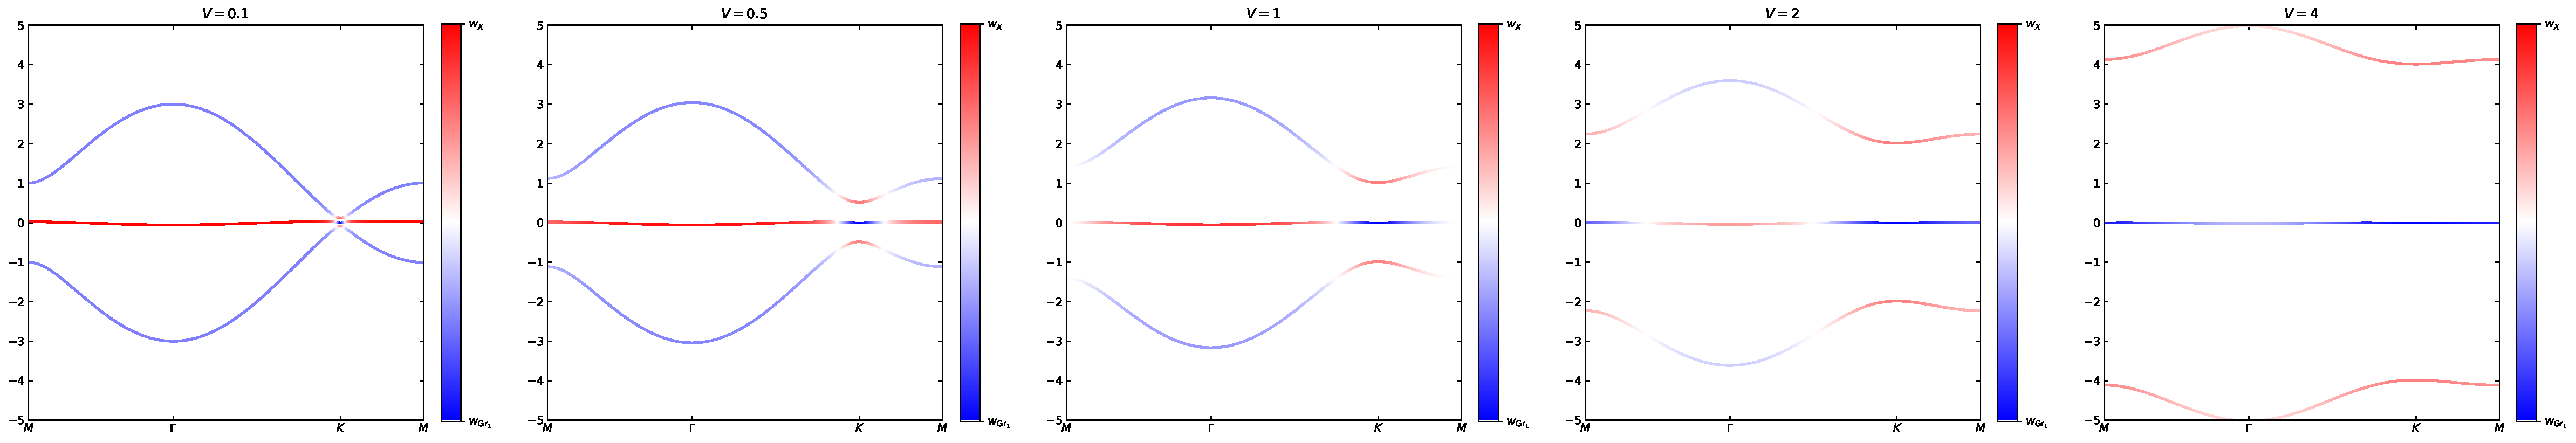
\includegraphics[width=\textwidth]{images/EG_X bands_tGr_1_tX_0.01}
    \caption{Bands of the non-interacting EG-X model. All the bands are spin-degenerate.}
    \label{fig:EG-X model non-interacting bands}
\end{figure}

\section{BCS Theory on the EG-X Model}\label{sec:bcs-theory-on-the-eg-x-model}

\subsection{BdG Hamiltonian}

Define sublattice index
\begin{equation}
    \alpha = 1, 2, 3
\end{equation}
with \(1 \hateq \mathrm{Gr}_1, 2 \hateq \mathrm{Gr}_2, 3 \hateq \mathrm{X}\).
Then we can write the non-interacting term as
\begin{equation}
    H_0 = - \sum_{\langle i, j \rangle, \alpha, \beta, \sigma} \left[\mat{t} \right]_{i\alpha,j\beta} c_{i\alpha}^{\dagger} c_{j\beta}
\end{equation}
with the matrix \todo{Does that make sense?}
\begin{equation}
    \mat{t} = \begin{pmatrix}
                  0 & t_{\mathrm{Gr}} & 0 \\
                  t_{\mathrm{Gr}} & 0 & -V \delta_{ij} \\
                  0 & -V \delta_{ij} & t_{\mathrm{X}} \\
    \end{pmatrix}
\end{equation}

Add chemical potential (to control filling \(n = \frac{N_{\uparrow} + N_{\downarrow}}{N_{\mathrm{sites}}}\) ):
\begin{equation}
    -\mu \sum_{i \alpha \sigma} n_{i \alpha \sigma}
\end{equation}

Also write the interaction part with \(\alpha\) (with changed signs -> to keep in line with papers about the attractive Hubbard model):
\begin{equation}
    H_{int} = - \sum_{i \alpha} U_{\alpha} c_{i\alpha \uparrow}^{\dagger} c_{i\alpha \downarrow}^{\dagger} c_{i\alpha \downarrow} c_{i\alpha \uparrow}
\end{equation}
Fourier transformation:
\begin{equation}
    H_{int} = - \frac{1}{N^2} \sum_{\alpha, \vb{k}_{1, 2, 3, 4}} U_{\alpha} e^{\iu (\vb{k}_1 + \vb{k}_4 - \vb{k}_1 - \vb{k}_3) r_{i \alpha}}  c_{\vb{k}_1 \alpha \uparrow}^{\dagger} c_{\vb{k}_3 \alpha \downarrow}^{\dagger} c_{\vb{k}_2 \alpha \downarrow} c_{\vb{k}_4 \alpha \uparrow}
\end{equation}
Imposing zero-momentum pairing: \(\vb{k}_1 + \vb{k}_3 = 0\) and \(\vb{k}_2 + \vb{k}_4 = 0\):
\begin{align}
    H_{int} = - \sum_{\alpha, \vb{k}, \vb{k}^{\prime}} U_{\alpha} c_{\vb{k} \alpha \uparrow}^{\dagger} c_{-\vb{k} \alpha \downarrow}^{\dagger} c_{-\vb{k}^{\prime} \alpha \downarrow} c_{\vb{k}^{\prime} \alpha \uparrow}
\end{align}
Mean-field approximation:
\begin{align}
    H_{int} \approx \sum_{\alpha, \vb{k}} (\Delta_{\alpha} c_{\vb{k} \alpha \uparrow}^{\dagger} c_{-\vb{k} \alpha \downarrow}^{\dagger} + \Delta_{\alpha}^* c_{-\vb{k} \alpha \downarrow} c_{\vb{k} \alpha \uparrow})
\end{align}
with
\begin{align}
    \Delta_{\alpha} &= - U_{\alpha} \sum_{\vb{k}^{\prime}} \braket{c_{-\vb{k}^{\prime} \alpha \downarrow} c_{\vb{k}^{\prime} \alpha \uparrow}} \\
    \Delta_{\alpha}^* &= - U_{\alpha} \sum_{\vb{k}^{\prime}} \braket{c_{\vb{k}^{\prime} \alpha \uparrow}^{\dagger} c_{-\vb{k}^{\prime} \alpha \downarrow}^{\dagger}}
\end{align}
This gives the BCS mean field Hamiltonian:
\begin{align}
    H_{BCS} =
\end{align}

with Nambu spinor
\begin{equation}
    \Psi_{\vb{k}} =
    \begin{pmatrix}
        c_{1, \vb{k} \uparrow} \\
        c_{2, \vb{k} \uparrow} \\
        c_{3, \vb{k} \uparrow} \\
        c_{1, -\vb{k} \downarrow}^{\dagger} \\
        c_{2, -\vb{k} \downarrow}^{\dagger} \\
        c_{3, -\vb{k} \downarrow}^{\dagger} \\
    \end{pmatrix}
\end{equation}
we have:
\begin{equation}
    H_{MF} = \sum_{\vb{k}} \Psi_{\vb{k}}^{\dagger} \mathcal{H} (\vb{k}) \Psi_{\vb{k}}
\end{equation}
with
\begin{equation}
    \mathcal{H} (\vb{k}) =
    \begin{pmatrix}
        H_{0, \uparrow} - \mu & \Delta \\
        \Delta^{\dagger} & - H_{0, \downarrow}^* (-\vb{k}) + \mu
    \end{pmatrix}
\end{equation}
with \(H_{0, \sigma}\) being the F.T. of the kinetic term and \(\Delta = diag(\Delta_1, \Delta_2, \Delta_3)\).

\subsection{BdG Hamiltonian in band basis}

Use transformation
\begin{equation}
    G =
\end{equation}
where the is made up of the eigenvectors of \(\mat{H}_{\sigma}\) for a given \(\vb{k}\):
\begin{equation}
    \mat{G} = 
    \begin{pmatrix}
        \vb{G}_1 & \vb{G}_2 & \vb{G}_3
    \end{pmatrix}
\end{equation}

with that:
\begin{equation}
    \mat{G}^{\dagger}_{\sigma} (\vb{k}) \mat{H}_{\sigma} (\vb{k}) \mat{G}_{\sigma} (\vb{k}) =
    \begin{pmatrix}
        \epsilon_1 & 0 & 0 \\
        0 & \epsilon_2 & 0 \\
        0 & 0 & \epsilon_3
    \end{pmatrix}
\end{equation}

So the 


\subsection{Self-consistent calculation of the superconducting gaps}

Compare~\cite[ch. 10]{Bruus_Flensberg_2004}.
Notable here: Multiple bands, and the gaps in each band depend in a complicated manner on the parameters \(U_{\alpha}\) and the orbital Green's functions.

Define normal Green's function:
\begin{equation}
    \mathcal{G}_{n\uparrow n\uparrow} (\vb{k}, \tau) = -\braket{T_{\tau} d_{n \vb{k} \uparrow} (\tau) d_{n \vb{k} \uparrow}^{\dagger} (0)}
\end{equation}
Anomalous Green's function:
\begin{equation}
    \mathcal{F}_{n\downarrow n\uparrow} (\vb{k}, \tau) = -\braket{T_{\tau} d_{n -\vb{k} \downarrow} (\tau) d_{n \vb{k} \uparrow}^{\dagger} (0)}
\end{equation}

Equations of motion (Heisenberg equation), follow~\cite[ch. 17]{Bruus_Flensberg_2004}:
\begin{align}
    \pdif{\tau} \mathcal{G}_{n\uparrow n\uparrow} (\vb{k}, \tau) &= -\delta (\tau) + \braket{T_{\tau} \left[d_{n \vb{k} \uparrow}, H\right] (\tau) d_{n \vb{k} \uparrow}^{\dagger} (0)} \\
    \pdif{\tau} \mathcal{F}_{n\downarrow n\uparrow} (\vb{k}, \tau) &= \braket{T_{\tau} \left[d_{n -\vb{k} \downarrow}, H\right] (\tau) d_{n \vb{k} \uparrow}^{\dagger} (0)}
\end{align}

Calculate the commutators:
\begin{align}
    \left[ d \right]
\end{align}

All in all:
\begin{align}
    \pdif{\tau} \mathcal{G}_{n \uparrow n \uparrow} (\vb{k}, \tau) &= -\delta(\tau) - \xi_{n \vb{k}} \mathcal{G}_{n \uparrow n \uparrow} (\vb{k}, \tau) + \Delta_{n} \mathcal{F}_{n\downarrow n\uparrow} (\vb{k}, \tau) \\
    \pdif{\tau} \mathcal{F}_{n \downarrow n \uparrow} (\vb{k}, \tau) &= \xi_{n \vb{k}} \mathcal{F}_{n \downarrow n \uparrow} (\vb{k}, \tau) + \Delta_{n}^* \mathcal{G}_{n\downarrow n\uparrow} (\vb{k}, \tau)
\end{align}
Fourier transform:
\begin{align}
    (-\iu \omega_n + \xi_{n \vb{k}}) \mathcal{G}_{n \uparrow n \uparrow} (\vb{k}, \iu \omega_n) &= -1 + \Delta_{n} \mathcal{F}_{n\downarrow n\uparrow} (\vb{k}, \iu \omega_n) \\
    (-\iu \omega_n - \xi_{n \vb{k}}) \mathcal{F}_{n \downarrow n \uparrow} (\vb{k}, \iu \omega_n) &= \Delta_{n}^* \mathcal{G}_{n\downarrow n\uparrow} (\vb{k}, \iu \omega_n)
\end{align}
This algebraic expression can be easily solved:
\begin{align}
    (-\iu \omega_n - \xi_{n \vb{k}}) \mathcal{F}_{n \downarrow n \uparrow} (\vb{k}, \iu \omega_n) &= \frac{\Delta_{n}^*}{-\iu \omega_n + \xi_{n \vb{k}}} (-1 + \Delta_{n} \mathcal{F}_{n\downarrow n\uparrow} (\vb{k}, \iu \omega_n))
\end{align}
\begin{align}
    (-\iu \omega_n - \xi_{n \vb{k}} - \frac{\vert\Delta_{n}\vert^2}{-\iu \omega_n + \xi_{n \vb{k}}}) \mathcal{F}_{n \downarrow n \uparrow} (\vb{k}, \iu \omega_n) &= \frac{-\Delta_{n}^*}{-\iu \omega_n + \xi_{n \vb{k}}} \\
    (\frac{(-\iu \omega_n - \xi_{n \vb{k}} )(-\iu \omega_n + \xi_{n \vb{k}}) - \vert\Delta_{n}\vert^2}{-\iu \omega_n + \xi_{n \vb{k}}}) \mathcal{F}_{n \downarrow n \uparrow} (\vb{k}, \iu \omega_n) &= \frac{-\Delta_{n}^*}{-\iu \omega_n + \xi_{n \vb{k}}}
\end{align}
\begin{align}
    \mathcal{F}_{n \downarrow n \uparrow} (\vb{k}, \iu \omega_n) &= \frac{-\Delta_{n}^*}{(-\iu \omega_n - \xi_{n \vb{k}} )(-\iu \omega_n + \xi_{n \vb{k}}) - \vert\Delta_{n}\vert^2} \\
    &= \frac{-\Delta_{n}^*}{(\iu \omega_n)^2 - \xi_{n \vb{k}}^2 - \vert\Delta_{n}\vert^2} \\
    &= \frac{-\Delta_{n}^*}{(\iu \omega_n)^2 - E_{n \vb{k}}}
\end{align}
\begin{align}
    (-\iu \omega_n + \xi_{n \vb{k}}) \mathcal{G}_{n \uparrow n \uparrow} (\vb{k}, \iu \omega_n) &= -1 + \frac{-\vert\Delta_{n}\vert^2}{(\iu \omega_n)^2 - \xi_{n \vb{k}}^2 - \vert\Delta_{n}\vert^2} \\
    &= \frac{-(\iu \omega_n)^2 + \xi_{n \vb{k}}^2 + \vert\Delta_{n}\vert^2 -\vert\Delta_{n}\vert^2}{(\iu \omega_n)^2 - \xi_{n \vb{k}}^2 - \vert\Delta_{n}\vert^2} \\
    &= \frac{-(\iu \omega_n)^2 + \xi_{n \vb{k}}^2}{(\iu \omega_n)^2 - \xi_{n \vb{k}}^2 - \vert\Delta_{n}\vert^2} \\
    &= \frac{(\iu \omega_n + \xi_{n \vb{k}})(-\iu \omega_n + \xi_{n \vb{k}})}{(\iu \omega_n)^2 - \xi_{n \vb{k}}^2 - \vert\Delta_{n}\vert^2}
\end{align}
\begin{align}
    \mathcal{G}_{n \uparrow n \uparrow} (\vb{k}, \iu \omega_n) &= \frac{\iu \omega + \xi_{n \vb{k}}}{(\iu \omega_n)^2 - \xi_{n \vb{k}}^2 - \vert\Delta_{n}\vert^2} \\
    &= \frac{\iu \omega + \xi_{n \vb{k}}}{(\iu \omega_n)^2 - E_{n \vb{k}}}
\end{align}
with the energies \(E_{n \vb{k}} = \pm \sqrt{\xi_{n \vb{k}}^2 - \vert\Delta_{n}\vert^2}\).

To calculate the band gap in band \(n\):
\begin{align}
    \Delta_n (\vb{k}) &= -\sum_{\alpha} [G_{k \uparrow}]_{\alpha n}^* \Delta_{\alpha} [G_{-k \downarrow}]_{\alpha n}^* \\
    &= -\sum_{\alpha \vb{k}^{\prime}} U_{\alpha} [G_{k \uparrow}]_{\alpha n}^* \braket{c_{-k^{\prime} \alpha \downarrow} c_{k^{\prime} \alpha \uparrow}} [G_{-k \downarrow}]_{\alpha n}^* \\
    &= -\sum_{\alpha \vb{k}^{\prime}} U_{\alpha} [G_{k \uparrow}]_{\alpha n}^* [G_{-k \downarrow}]_{\alpha n}^* \sum_{m} [G_{-k^{\prime} \downarrow}]_{\alpha m} [G_{k^{\prime} \uparrow}]_{\alpha m} \braket{d_{-k^{\prime} m \downarrow} d_{k^{\prime} m \uparrow}}
\end{align}
Can now use \(\mathcal{F}\) and fourier-transform:
\begin{align}
    \braket{d_{-k^{\prime} m \downarrow} d_{k^{\prime} m \uparrow}} &= \mathcal{F}_{m \downarrow m \uparrow}^* (\vb{k}^{\prime}, \tau = 0^+) \\
    &= \frac{1}{\beta} \sum_{\iu \omega_n} e^{-\iu \omega_n 0^+} \mathcal{F}_{m \downarrow m \uparrow}^* (\vb{k}^{\prime}, \iu \omega_n)
\end{align}
The summation over the Matsubara frequencies can be solved via the Residue theorem (the poles \(z_0\) of \(\mathcal{F}\) are the energies \(\pm E_{m \vb{k}}\)):
\begin{align}
    &\frac{1}{\beta} \sum_{\iu \omega_n} e^{-\iu \omega_n 0^+} \mathcal{F}_{m \downarrow m \uparrow}^* (\vb{k}^{\prime}, \iu \omega_n) \\
    &= \sum_{z_0 \text{poles of} \mathcal{F}} e^{-z_0 0^+} n_{F} (z_0) Res_{z_0} \mathcal{F}_{m \downarrow m \uparrow}^*  (\vb{k}^{\prime}, z_0) \\
    &= e^{-E_{m \vb{k}} 0^+} n_{F} (E_{m \vb{k}}) Res_{E_{m \vb{k}}} \frac{-\Delta_{m}^*}{(\iu \omega_n)^2 - E_{m \vb{k}}}
    + e^{E_{m \vb{k}} 0^+} n_{F} (-E_{m \vb{k}}) Res_{-E_{m \vb{k}}} \frac{-\Delta_{m}^*}{(\iu \omega_n)^2 - E_{m \vb{k}}}
\end{align}
with residue:
\begin{equation}
    Res_{E_{m \vb{k}}} \frac{1}{(\iu \omega_n)^2 - z_0^2} = \frac{1}{\pdif{z}\vert_{z_0 = E_{m \vb{k}}} ((\iu \omega)^2 - z_0^2)} = \frac{1}{2 E_{m \vb{k}}}
\end{equation}
So we have
\begin{align}
    \braket{d_{-k^{\prime} m \downarrow} d_{k^{\prime} m \uparrow}} &= -\Delta_m^* \left(\frac{n_F (E_{m \vb{k}})}{2 E_{m \vb{k}}} - \frac{n_F (-E_{m \vb{k}})}{2 E_{m \vb{k}}}\right)
\end{align}
